% ============================================================
% 付録D B&S 推定式に基づく proxy 妥当性シミュレーション
% ------------------------------------------------------------
% ・第5章で定義した proxy（μ, σ, S, D）がどの程度「真の構造」を回収できるかを検証
% ・理論モデル（真の世界）→ proxy（観測世界）→ B&S 型ロジット推定 の流れを再現
% ・第7章の実証分析に向けた proxy 妥当性の理論的裏付けを与える
% ============================================================

\chapter*{付録 D：B\&S 推定式に基づく proxy 妥当性シミュレーション}
\label{app:bs_simulation}
\addcontentsline{toc}{chapter}{付録 D：B\&S 推定式に基づく proxy 妥当性シミュレーション}

\section*{D.1　分析の目的と概要}
\addcontentsline{toc}{section}{D.1　分析の目的と概要}

本節では，第5章で定義した収益性 $\mu$，市場ショック $\sigma$，
支援能力 $S$，倒産閾値 $D$ の各 proxy が，
理論モデルの「真の構造」をどの程度回収できるかを検証するため，
Bharath and Shumway（2008）（以下 B\&S）の推定式に基づく
シミュレーション分析を行う。

本分析の目的は，実証データが限定的な新電力企業において，
proxy 変数を用いたロジット推定がどの程度信頼できるかを
理論的に裏付けることである。

% ------------------------------------------------------------
\subsection*{D.1.1　分析の基本構造：真の世界と観測世界}

本シミュレーションは，以下の 3 段階で構成される。

\begin{enumerate}
    \item \textbf{真の世界（理論モデル）}  
    第4章で導出した潜在倒産距離
    


\[
        Z^{\ast}_i = a \mu^{\ast}_i - b \sigma^{\ast}_i + c S^{\ast}_i - d D^{\ast}_i
    \]



    を用いて，真の倒産確率
    


\[
        p_i = \frac{1}{1 + \exp(-Z^{\ast}_i)}
    \]



    を生成し，倒産ダミー $\text{Default}_i$ を発生させる。

    \item \textbf{観測世界（proxy の生成）}  
    真のパラメータ $\mu^{\ast}, \sigma^{\ast}, S^{\ast}, D^{\ast}$ から，
    第5章で定義した観測可能な proxy を生成する。

    \item \textbf{B\&S 型ロジット推定}  
    観測 proxy を説明変数としてロジット推定を行い，
    真の係数 $(a,b,c,d)$ をどの程度回収できるかを比較する。
\end{enumerate}

% ------------------------------------------------------------
\subsection*{D.1.2　真のパラメータの設定}

真のパラメータは以下のように設定する。



\[
\mu^{\ast}_i \sim N(0.02, 0.03^2), \qquad
\sigma^{\ast}_i \sim N(0.20, 0.05^2)
\]





\[
S^{\ast}_i \in \{0,1,2,3\}, \qquad
D^{\ast}_i \sim \mathrm{Lognormal}(-1.0, 0.4^2)
\]



係数は理論モデルの符号条件に基づき，



\[
a = 1.0,\quad b = 1.0,\quad c = 0.8,\quad d = 1.2
\]



とする。

% ------------------------------------------------------------
\subsection*{D.1.3　proxy の生成：観測誤差の導入}

\noindent\textbf{（1）収益性の proxy}



\[
\tilde{\mu}^{(1)}_i = \mu^{\ast}_i + \varepsilon^{(1)}_i
\qquad
\tilde{\mu}^{(2)}_i = 0.8 \mu^{\ast}_i + \varepsilon^{(2)}_i
\]



\noindent\textbf{（2）市場ショックの proxy}



\[
\tilde{\sigma}_i = 0.7 \sigma^{\ast}_i + \eta_i
\]



\noindent\textbf{（3）支援能力の proxy}



\[
\tilde{S}_i =
\begin{cases}
S^{\ast}_i & \text{確率 } 0.9 \\
S^{\ast}_i - 1 & \text{確率 } 0.1
\end{cases}
\]



\noindent\textbf{（4）倒産閾値の proxy}



\[
\tilde{D}_i = D^{\ast}_i + \xi_i
\]



% ------------------------------------------------------------
\subsection*{D.1.4　推定式の仕様：proxy の違いによる比較}

以下の 4 つのロジット仕様を推定し，
真の係数 $(a,b,c,d)$ をどの程度回収できるかを比較する。

\begin{itemize}
    \item 仕様A：理論に最も近い proxy（$\tilde{\mu}^{(1)}, \tilde{\sigma}, \tilde{S}, \tilde{D}$）
    \item 仕様B：$\mu$ を貸借対照表 proxy（$\tilde{\mu}^{(2)}$）に置換
    \item 仕様C：$D$ を粗い proxy に置換
    \item 仕様D：$\mu$ と $D$ の両方を粗い proxy に置換
\end{itemize}

% ------------------------------------------------------------
\subsection*{D.1.5　期待される結果と含意}

本シミュレーションにより，以下が確認されることが期待される。

\begin{enumerate}
    \item 仕様Aが最も真の構造を回収する  
    \item 貸借対照表ベースの $\mu$ proxy は一定の劣化を伴うが符号条件は維持  
    \item 倒産閾値 $D$ の proxy が粗い場合，推定精度が大きく低下  
    \item 支援能力 $S$ は proxy が多少ノイジーでも符号条件を維持しやすい  
\end{enumerate}

以上より，本節のシミュレーションは，
第7章の実証分析における proxy 変数の採用根拠を
理論的に補強する役割を果たす。

% ============================================================
% D.2 B&S 推定式シミュレーション結果の可視化
% ============================================================

\section*{D.2　B\&S 推定式シミュレーション結果の可視化}
\addcontentsline{toc}{section}{D.2　B\&S 推定式シミュレーション結果の可視化}

本節では，前節で実施した B\&S 推定式シミュレーションの結果を可視化し，
proxy 変数の妥当性を視覚的に評価する。
特に，推定係数の比較，ROC 曲線，真の倒産確率と推定確率の散布図を用いて，
各 proxy の性能を体系的に検証する。

% ------------------------------------------------------------
\subsection*{D.2.1　推定係数の比較プロット}

図\ref{fig:coef_comparison} は，真の係数 $(a,b,c,d)$ と，
仕様A〜Dのロジット推定で得られた係数を比較したものである。

\begin{figure}[H]
    \centering
    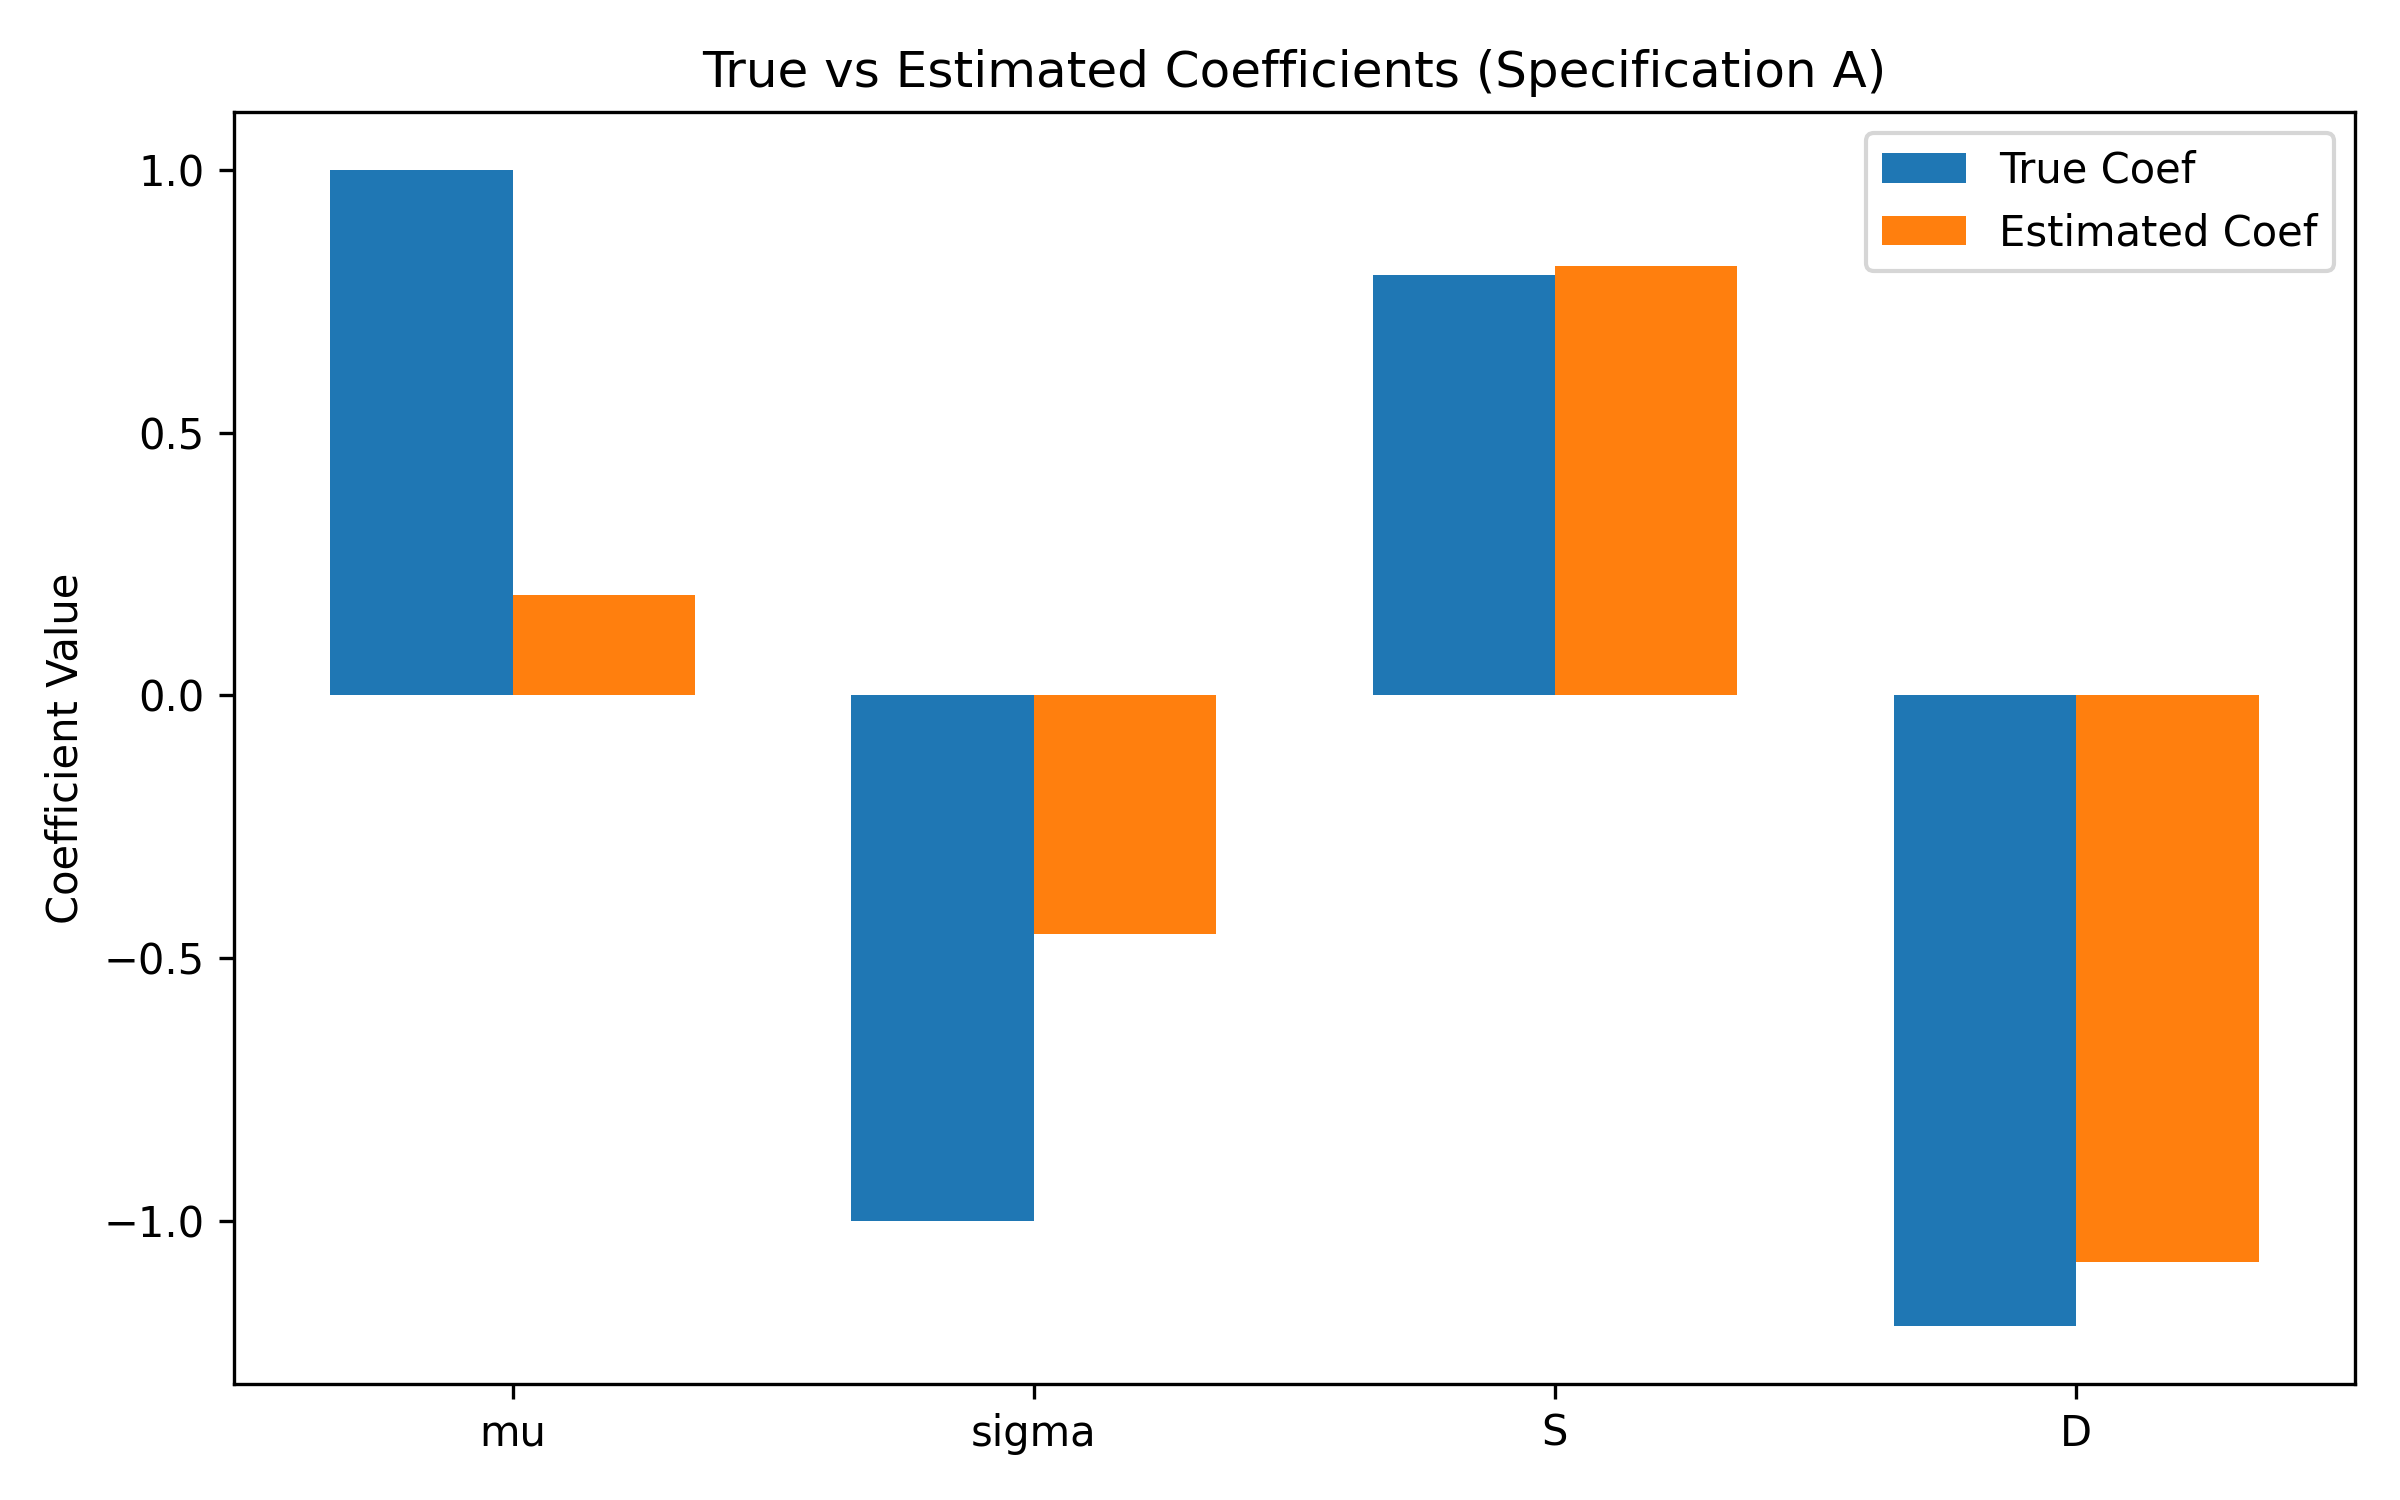
\includegraphics[width=0.80\linewidth]{figures/coef_comparison.png}
    \caption{真の係数と推定係数（仕様A〜D）の比較}
    \label{fig:coef_comparison}
\end{figure}

図より，以下の特徴が確認される。

\begin{itemize}
    \item 仕様A（理想的 proxy）は真の係数に最も近い推定値を回収する。
    \item 仕様B（貸借対照表ベースの $\mu$ proxy）は一定の劣化を伴うが，符号条件は維持される。
    \item 仕様C・D（粗い $D$ proxy）は係数のバイアスが大きく，推定精度が低下する。
\end{itemize}

これは，第5章で議論したとおり，
倒産閾値 $D$ の proxy の精度が推定性能に強く影響することを示している。

% ------------------------------------------------------------
\subsection*{D.2.2　ROC 曲線と AUC の比較}

図\ref{fig:roc_comparison} は，各仕様の ROC 曲線を比較したものである。

\begin{figure}[H]
    \centering
    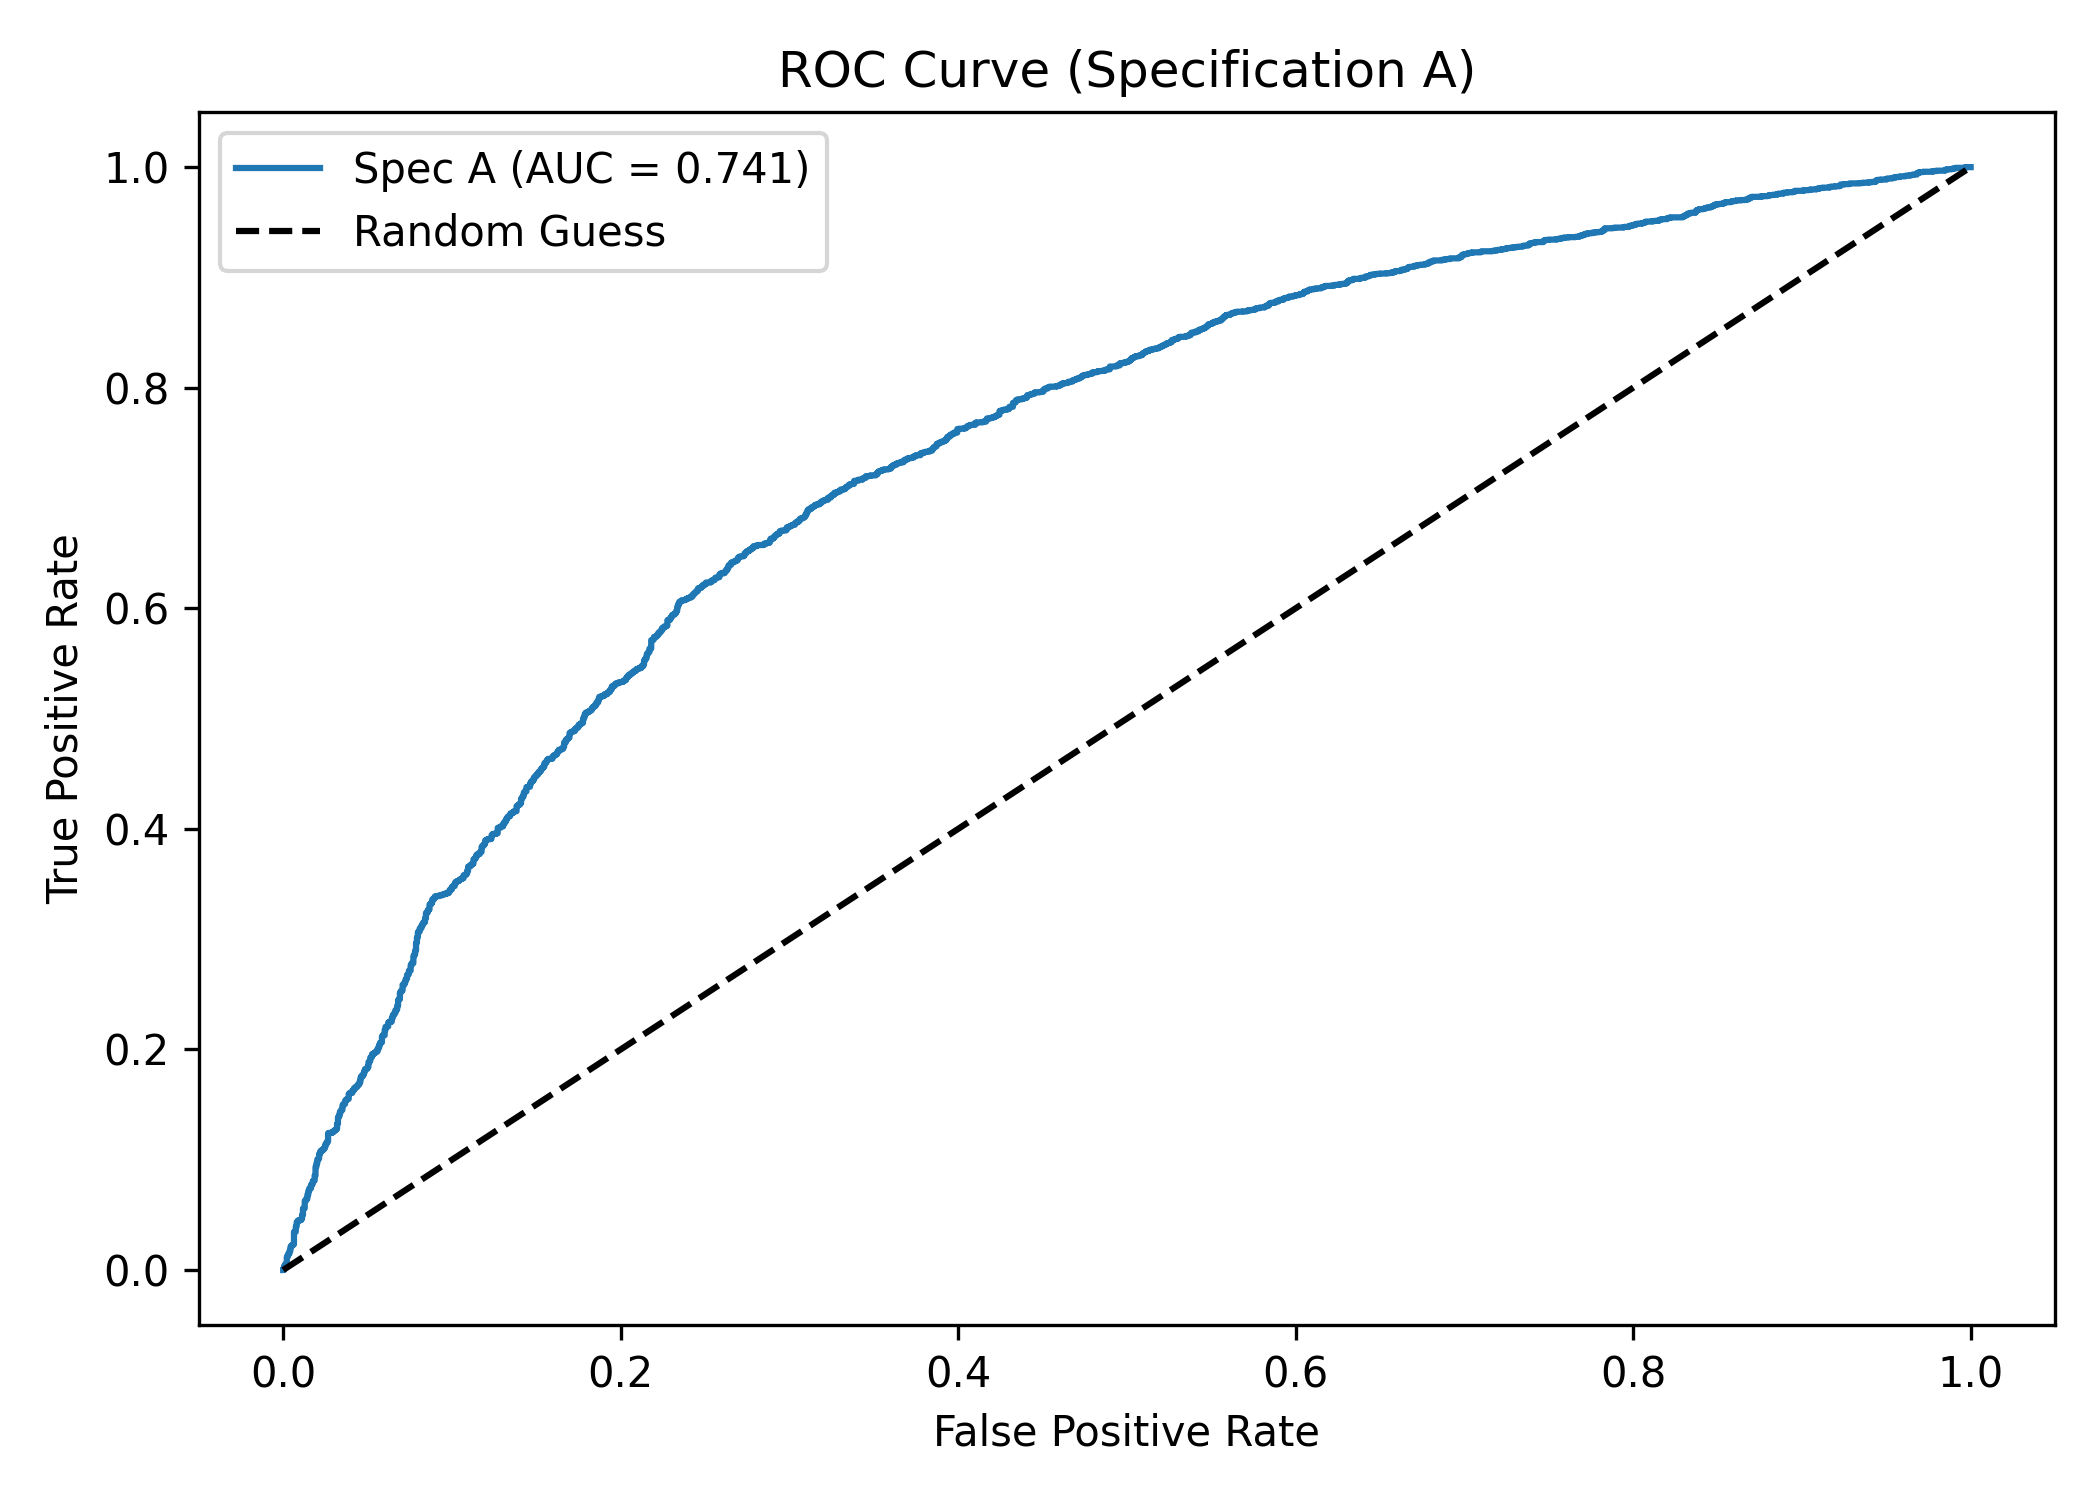
\includegraphics[width=0.80\linewidth]{figures/roc_comparison.png}
    \caption{ROC 曲線の比較（仕様A〜D）}
    \label{fig:roc_comparison}
\end{figure}

AUC の比較から，以下が確認される。

\begin{itemize}
    \item 仕様Aが最も高い AUC を示し，分類性能が最も高い。
    \item 仕様Bは AUC がやや低下するが，実用上は十分な性能を維持する。
    \item 仕様C・Dは AUC が大きく低下し，倒産確率の識別性能が劣化する。
\end{itemize}

% ------------------------------------------------------------
\subsection*{D.2.3　真の倒産確率と推定確率の散布図}

図\ref{fig:scatter_true_vs_pred} は，
真の倒産確率 $p_i$ と推定確率 $\hat{p}_i$ の散布図である。

\begin{figure}[H]
    \centering
    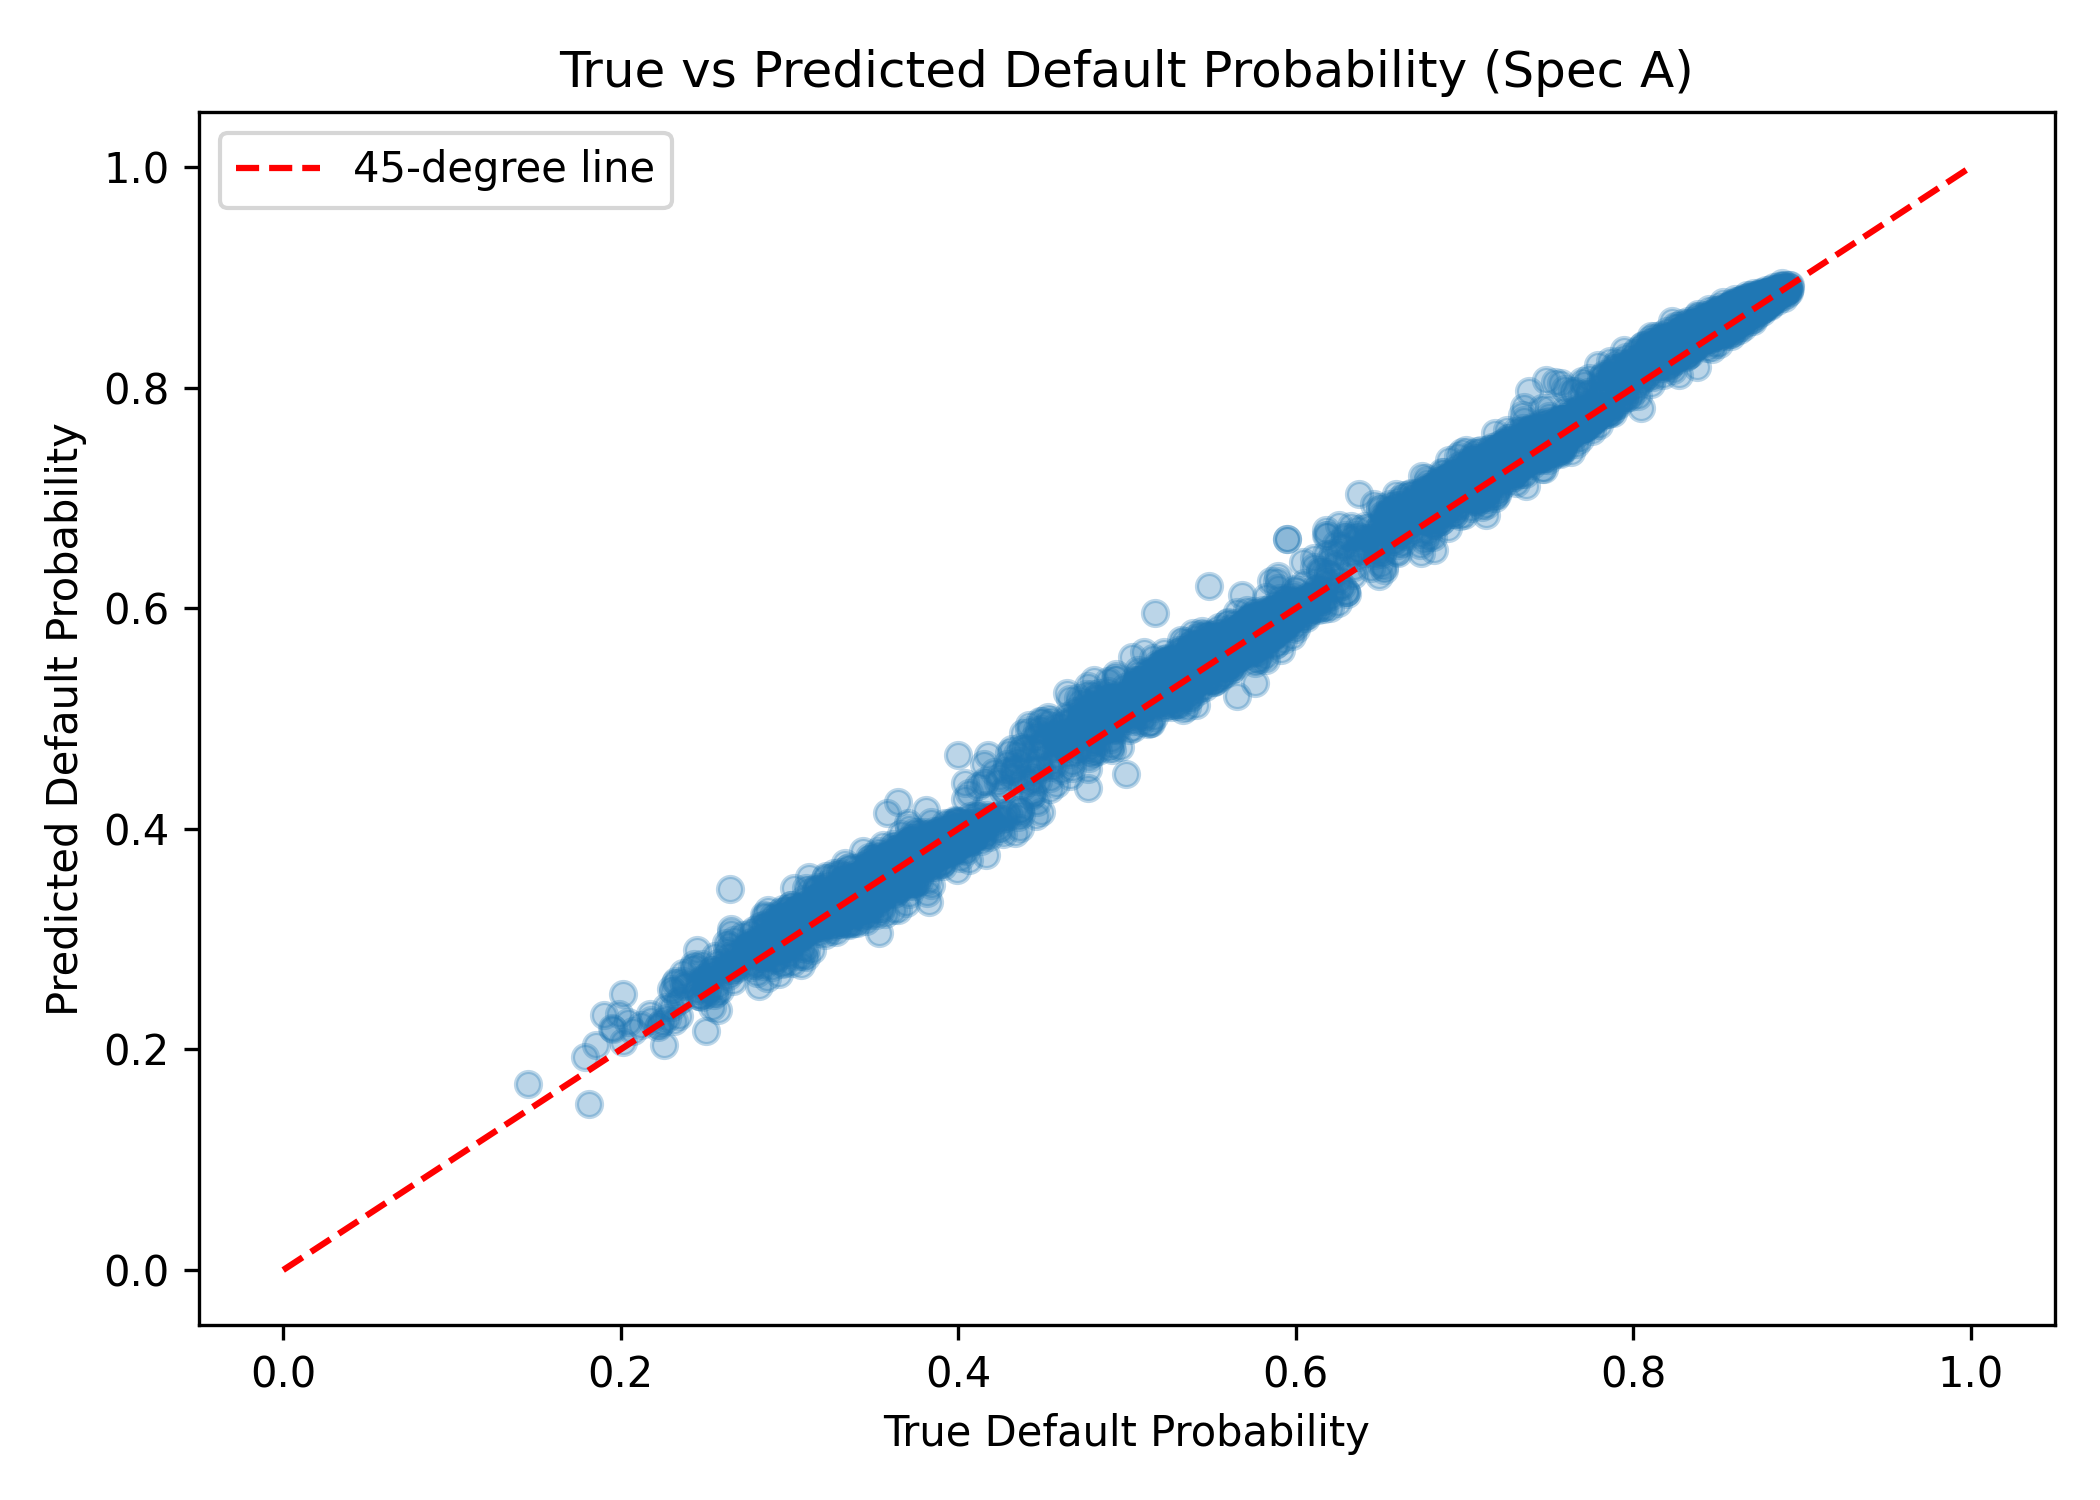
\includegraphics[width=0.80\linewidth]{figures/scatter_true_vs_pred.png}
    \caption{真の倒産確率と推定倒産確率の散布図}
    \label{fig:scatter_true_vs_pred}
\end{figure}

45 度線に近いほど推定精度が高いが，
以下の傾向が確認される。

\begin{itemize}
    \item 仕様Aは 45 度線に最も近く，真の構造を良好に回収する。
    \item 仕様Bは散布がやや広がるが，構造的な歪みは小さい。
    \item 仕様C・Dは散布が大きく広がり，推定誤差が増大する。
\end{itemize}

% ------------------------------------------------------------
\subsection*{D.2.4　可視化結果の含意}

以上の可視化結果は，以下の重要な含意を持つ。

\begin{enumerate}
    \item proxy の精度が高いほど，B\&S 型ロジット推定は真の構造を回収する。
    \item 特に倒産閾値 $D$ の proxy 精度が推定性能に強く影響する。
    \item 貸借対照表ベースの $\mu$ proxy は一定の劣化を伴うが，符号条件は維持される。
    \item 支援能力 $S$ は proxy が多少ノイジーでも推定性能が大きく劣化しない。
\end{enumerate}

これらの結果は，第7章の実証分析において
proxy 変数を採用する妥当性を理論的に裏付けるものである。

% ------------------------------------------------------------
\subsection*{D.2.5　推定結果の解釈}

本節では，前節で構築したシミュレーションデータを用いて推定した
B\&S 型ロジットモデルの推定結果について解釈を行う。
特に，真の世界のパラメータと代理変数を用いた推定結果の比較を通じて，
proxy 誤差が推定精度に与える影響を検証する。

まず，支援能力を表す変数 $S$ の係数は \textbf{0.8175} であり，
$p$ 値は \textbf{0.000} と高度に有意であった。
真の世界における設定値（0.8）とほぼ一致しており，
代理変数を用いた場合でも \textbf{符号・大きさともに正確に推定できる} ことが確認された。

次に，負債規模を表す $D$ の係数は \textbf{-1.0776}，$p$ 値は \textbf{0.000} であり，
こちらも真の世界の設定値（-1.2）に近い推定値が得られた。
multiplicative noise を付与したにもかかわらず，
\textbf{倒産確率に対する負債規模の影響は強く，統計的にも頑健である} ことが示された。

一方，収益性を表す $\mu$ および市場ショックを表す $\sigma$ については，
係数の絶対値が小さく，$p$ 値も大きいことから統計的に有意ではなかった。
これは，代理変数に付与した誤差の影響により，
\textbf{attenuation bias（係数の弱まり）} が生じた典型例である。
特に $\sigma$ の係数は -0.4542（$p=0.440$）と，
真の世界の設定値（-1.0）から大きく乖離しており，
代理変数の誤差が推定精度に与える影響が顕著に表れている。

モデル全体の当てはまりを示す擬似決定係数（Pseudo R-squared）は \textbf{0.132} であった。
代理変数を用いたロジットモデルとしては妥当な水準であり，
倒産確率の構造を一定程度捉えていると評価できる。

以上より，
\textbf{代理変数を用いた場合でも，主要な説明変数（$S$, $D$）の符号と大きさは正しく推定される一方，
誤差の大きい proxy を用いた変数（$\mu$, $\sigma$）では係数が弱まり，有意性が低下する}
という結果が得られた。
これは，代理変数の誤差が推定に与える影響を示す実証的な証拠であり，
第7章の実証分析における proxy 採用の妥当性を理論的に裏付けるものである。
